% ============================================================
% arXiv Submission — RoboParts: Three-State Honesty
% Template: plain LaTeX article (arXiv-friendly, no elsarticle dependency)
% Compile: pdflatex main.tex && bibtex main && pdflatex x2
% ============================================================
\documentclass[11pt,twocolumn]{article}
\usepackage[margin=0.9in]{geometry}
\usepackage{amsmath,amssymb,amsfonts}
\usepackage{graphicx}
\usepackage{booktabs}
\usepackage{xcolor}
\usepackage{hyperref}
\usepackage{url}
\usepackage{array}
\usepackage{enumitem}
\usepackage{microtype}

% arXiv DOI line — will be filled by arXiv after first publication
\usepackage{fancyhdr}
\pagestyle{plain}

% ============================================================
% Title & Authors
% ============================================================
\title{Three-State Honesty in Robotic Hardware Compatibility:\\
       A Vendor-Neutral Determination Layer
  \vspace{0.4cm}
  \begin{flushright}
    \footnotesize
    \texttt{arXiv:XXXX.XXXXX [cs.AI]} \\
    Code: \url{https://github.com/lm203688/roboparts} \\
    Data: CC BY 4.0 \quad Code: MIT
  \end{flushright}
}

\author{Lexing Li \\
\textit{Independent Researcher, China} \\
\texttt{463102527@qq.com} \\
ORCID: \url{https://orcid.org/0009-0004-2152-7669}}

\date{\today}

% ============================================================
\begin{document}

\maketitle

\begin{abstract}
Compatibility determination between robotic hardware components is the
foundational yet most fragile step in the supply chain of embodied AI.
Existing engineering practice addresses ``can this part be mounted on
that?'' through three unsatisfactory routes: free-form documentation,
bill-of-materials and trial-and-error, or vendor-private compatibility
matrices. All three are binary --- either \emph{yes} or \emph{no} ---
although real engineering is filled with combinations that must be
labelled \emph{unknown}. The forced binary answer causes two symmetric
errors: false-positive compatibility (mechanical damage, personal
injury) and false-negative compatibility (wasted integration time).

We present \textbf{RoboParts}, a vendor-neutral determination layer
that formalises compatibility as a three-valued function over a
three-axis type system:
$\mathsf{compose}(a,b) \in \{\mathsf{composed}, \mathsf{type\_error}, \mathsf{unknown}\}$,
with the design choice that \emph{unknown} takes priority over
\emph{composed} --- ignorance is a first-class citizen, not a null value.
The mechanical axis inherits reflexivity (same standard implies
compatibility) only for \emph{geometric-spec} types; it is deliberately
withdrawn for \emph{directional-role} types (e.g.\ \texttt{OUTPUT\_SPIKE},
where two matching instances are not complementary). The electrical and
signal axes are evaluated independently.

Across $868$ real-world robotic entities yielding $430{,}336$ full
pair evaluations, we observe $\mathsf{composed}=0$,
$\mathsf{type\_error}=262$, $\mathsf{unknown}=430{,}074$ --- a coverage
map, not a benchmark failure. We introduce \emph{gap-distance} and
\emph{d1-bottleneck} measures that turn the $unknown$ mass into an
actionable data-flywheel priority queue: on our current snapshot,
$61$ pairs at $d=1$ split between electrical ($32$, $52.46\%$) and
signal ($29$, $47.54\%$) axes --- a two-axis bottleneck, not a single
one. A three-class gap causation taxonomy
(unpublished-suspect / proprietary-suspect / ambiguous) together with
a manufacturer concentration analysis shows that the top-$10$ of $358$
named vendors account for $37.33\%$ of the entity mass, ruling out
``crawl a few datasheets'' as a viable closure strategy and pointing
to user-submission and open-source-BOM reverse-feeding as the only
scalable paths.
\end{abstract}

\noindent\textbf{Keywords.}
Robotic hardware compatibility; vendor-neutral knowledge layer;
three-valued reasoning; engineering ontology;
data-flywheel prioritisation; knowledge-graph.

\section*{Declaration of generative AI and AI-assisted technologies}
\small
During the preparation of this manuscript, the authors used
\textbf{ChatGPT-4o} and \textbf{DeepSeek} for language editing and
figure captions only. All scientific claims, formalisations,
experiments, and dataset statistics were produced, verified, and
reproducible without AI assistance. All authors have reviewed and
approved the final manuscript and take full responsibility for
its content.

\section*{Declaration of competing interest}
The authors declare that they have no known competing financial
interests or personal relationships that could have appeared to
influence the work reported in this paper.

\section*{Data availability}
All data, code and intermediate artefacts used to produce the results
reported in this paper are released under MIT (code) and CC BY 4.0
(data) at \url{https://github.com/lm203688/roboparts}~\cite{roboparts-repo}. The dataset
snapshot referenced by this manuscript is anchored by the
\texttt{generated\_at} timestamp in each of the four API outputs
(\texttt{entities.json}, \texttt{gap\_classification.json},
\texttt{compose\_semantics.json}, \texttt{morphology\_graph.json}),
which are frozen at the revision named by that timestamp.

\section{Introduction}

The next bottleneck in embodied AI is not how smart a robot is, but
what it can be \emph{attached} to. A representative open-source arm
project (\textsc{Seeed reBot-DevArm}~\cite{R14}) publishes STEP files,
BOMs, a Python SDK, ROS\,2 integration, LeRobot tutorials and Isaac-Sim
simulations — four layers complete — but does not answer the question
``can this end-effector mount on this wrist, and can this sensor talk
to this mainboard?'' Compatibility determination has, for years,
lived as prose documentation, private vendor matrices, or manual
trial-and-error, with no neutral, machine-readable, decidable public
layer.

The central claim of this paper is that the correct semantics of
compatibility are not two-valued but \emph{three-valued}. ``I know
it works'' and ``I know it does not work'' are both evidence states;
``I do not know'' is a third evidence state, and it is the one that
tells you exactly which declaration to fill in and how many unknowns
that fills close. Ignoring this third state produces two symmetric,
costly errors:

\begin{itemize}[nosep,leftmargin=*]
\item \textbf{False-positive compatibility} — treating ``not found''
as ``yes'': mechanical damage, electrical failure, personal injury.
\item \textbf{False-negative compatibility} — treating ``not found''
as ``no'': hours of trial-and-error on combinations that in fact
work.
\end{itemize}

Our design principle is \emph{three-state honesty}: compatibility
is a function
\begin{equation}
  \mathsf{compose}(a, b) \;\in\;
  \{\mathsf{composed},\ \mathsf{type\_error},\ \mathsf{unknown}\}
  \label{eq:trivalue}
\end{equation}
where $\mathsf{unknown}$ \emph{outranks} $\mathsf{composed}$ — if
any of the three axes lacks evidence, the composite verdict is
$\mathsf{unknown}$. This is the sharp dividing line from every binary
compatibility matrix.

Vendor-neutrality is the second, non-negotiable design constraint:
RoboParts does not manufacture, resell, or take commission on any
part, and has no commercial tie to any listed vendor. A compatibility
layer with a monetary interest in one of the two queried parts has
an incentive to be wrong.

\paragraph{Contributions.}
\begin{enumerate}[nosep]
\item A three-valued compatibility function over a three-axis type
system (mechanical / electrical / signal), with an explicit
\emph{reflexivity boundary} — same-type means compatible only for
geometric-specification types (e.g.\ ISO 9409-1 flange sizes), and is
deliberately withdrawn for directional-role types
(\texttt{OUTPUT\_SPIKE}, \texttt{INPUT\_SENSORY}), where two matching
instances are complementary only if their roles differ.

\item A coverage map of $868$ robotic entities and $430{,}336$ full
pair evaluations yielding $16.2\%$ mechanical declaration rate
(deliberately reported as an \emph{honesty baseline} rather than
a benchmark; a stricter mechanical-decidability rate of $6.57\%$ is
reported under the standard-plus-flange joint-non-empty criterion).

\item Two new measures, \emph{gap-distance} ($d$ = number of axes
that returned $\mathsf{unknown}$ for a pair) and \emph{d1-bottleneck}
(axis responsible when $d=1$), which turn the $\mathsf{unknown}$ mass
into an actionable data-flywheel priority queue. On our current
corpus, the $61$ $d=1$ pairs are split between electrical ($32$)
and signal ($29$) axes --- the d1 bottleneck is a
\emph{two-axis} distribution, and we show that it shifts as evidence
is added (Section~\ref{sec:d1-shift}).

\item A three-class gap-causation taxonomy
(unpublished-suspect / proprietary-suspect / ambiguous) together with
a manufacturer concentration analysis ($358$ named vendors,
top-$10$ accounting for $37.33\%$ of the entity mass). This is
\emph{negative evidence}: the coverage gap cannot be closed by
crawling a small number of vendor datasheets. The only scalable paths
are user-submission, OSS-BOM reverse-feeding, and community pull-requests.

\item An engineering-verifiability harness of $78$ continuous-integration
gates with a documented mutation-kill rate of $82.1\%$ and a catalogue
of twelve verification anti-patterns (AP-01 to AP-12) with the first
six promoted to their own gates. This is the fourth contribution and
the one most directly transferable to any evidence-driven system: the
harness itself is a reusable artefact, the mutation-kill rate is an
honesty metric, and the anti-pattern ledger is the methodological
contribution that generalises across projects (Section~\ref{sec:eng-verif}).
\end{enumerate}

\paragraph{Paper outline.}
Section~2 surveys related work in assembly-graph learning, engineering
ontologies, and uncertainty-aware robot learning. Section~3 gives the
formal definitions. Section~4 describes the corpus. Section~5 reports
experiments. Section~6 discusses limitations and the reflexivity
boundary in depth. Section~7 concludes.

% ============================================================
% 2. Related Work
% ============================================================
\section{Related Work}

\subsection{Standards and the missing decision layer}

The three-axis backbone of RoboParts is deliberately thin on standards.
\textsc{ISO 9409-1}~\cite{iso9409} defines the canonical letter codes
(\texttt{A55} through \texttt{H350}) for the flange sizes used in
industrial manipulation devices. \textsc{ISO 3025}~\cite{iso3025}
fixes dowel-hole positions for those flanges. \textsc{ISO 9653}~\cite{iso9653}
covers safety-critical cylinder interfaces. What these standards
\emph{do not} define is the third axis — a signal-level type system
that lets two independently-produced devices be checked for whether
their roles are complementary. That gap is the reason that the
existence of a common flange is not sufficient to certify a mating
pair: two devices can share an \texttt{A55} flange and still be
electrical incompatible, or signal-direction incompatible.

We are not alone in wanting a machine-readable decision layer. The
\textsc{STEP-NC} framework for additive manufacturing~\cite{R12}
unifies geometry, material and process parameters into a single
digital spine, but at the \emph{manufacturing-process} scale, not the
selection-scale. \textsc{ANSI}'s survey of additive standards
\cite{R13} emphasises that standardisation has three components —
terminology alignment, data exchange, and test methods — and
that all three must be present for the layer to be useful. RoboParts
addresses terminology (three-axis type system), data exchange
(machine-readable \texttt{entities.json}), and test methods
(arithmetic crosscheck invariants) — but does not yet address the
\emph{calibration} step, which is the subject of Section~6.4.

\subsection{Assembly graphs and interface geometry}

The closest geometric neighbours to our work are assembly-graph
learners. Assembly graphs have emerged as a foundational
representation for learning-based assembly~\cite{AssemblyKG2022} and
continue to drive recent work on geometric interface reasoning.
\textsc{Linkify}~\cite{R1} re-computes high-fidelity contact points
for Fusion-360-Gallery assemblies and trains a GATv2 on top of
point-cloud encoded interfaces, achieving strong masked-part
prediction. Harlacher \& Friedrich~\cite{R2} learn geometric relation
labels from point clouds and then convert them into symbolic assembly
graphs, achieving $85.8\%$ success on \textsc{ASAP} with human-in-the-loop
correction. Semantic enrichment via LLM-annotated scene graphs over
CAD data~\cite{R3} takes the CAD-uncertainty direction: when the
annotator is uncertain, the annotator's uncertainty is preserved in
the graph. All three operate at the \emph{geometric} layer of
interfaces. RoboParts operates at the \emph{semantic} layer — types,
declarations, and unknowns — and is complementary to (not
competitive with) these methods. A geometry learner that trusts its
own point clouds can only ever tell you what it saw; RoboParts is
what tells you what it \emph{has not yet seen}.

A systematic study of machine learning on assembly guidance ontologies
\cite{R8} shows that AR-assisted assembly guidance benefits from
ontology-driven retrieval, but again operates on a fixed set of known
parts. \textsc{ExtruOnt}~\cite{R5} provides a formal ontology for
extrusion machines covering components, spatial connections, features
and sensors, and is a direct model of the ontology-driven approach we
adopt at the entity level. Ontology-based KGs for systems engineering
\cite{R6} and for robot manipulation with geometric constraints~\cite{R7}
both operate at the \emph{single-machine} scale. The unified graph
framework for industrial-robot automatic design~\cite{R4} pushes
toward design-time KGs that recommend parts — the dual of what we do
at query time. A systematic review of ontology-plus-ML research
\cite{R9} identifies this same cross-connection between ontology
definitions and downstream machine-learning pipelines, which is the
motivating background for RoboParts.

\subsection{Uncertainty-aware robot learning}

On the decision side, conformal prediction has become the dominant
distribution-free framework for uncertainty quantification in
robotics: adaptive conformal prediction has been integrated with
probabilistic control barrier functions for high-probability safety
guarantees~\cite{ACP2024}, learnable nonconformity scores tighten
prediction intervals in perception and planning tasks
\cite{LCP2025}, and local conformal calibration addresses the joint
aleatoric/epistemic gap under dynamics shift~\cite{LUCCa2024}.
\textsc{ReconVLA}~\cite{R10} uses conformal prediction intervals to
give vision-language-action policies explicit coverage guarantees,
letting the planner refuse when the interval is too wide. The VLA
uncertainty survey~\cite{R11} makes the same argument at a higher
level: a policy that returns \emph{I don't know} is strictly better
than one that guesses when guessing is more costly than deferring.
Resource-bounded type theory offers a dual formalisation of
compositional cost guarantees via abstract resource lattices
\cite{RBT2025}, which is the same ``unknown beats wrong'' discipline
applied to complexity rather than safety. RoboParts brings the same
three-valued philosophy to the \emph{data} layer rather than the
\emph{decision} layer. The stack reads bottom-up as: \emph{data layer
three-state (compatibility)} $\rightarrow$ \emph{reasoning layer KG
(assembly planning)} $\rightarrow$ \emph{decision layer UQ (policy
refusal)}. Each layer's unknown feeds the previous one's priority
queue.

\subsection{Open-source hardware and BOM semantics}

Two representative open-source arm/hand projects show the current
state of vendor-published hardware data. \textsc{Seeed reBot-DevArm}~\cite{R14}
ships STEP files, a BOM, Python SDK, ROS\,2 integration, LeRobot
tutorials, and Isaac-Sim simulations — but does not annotate any
interface on any part with a machine-readable type. \textsc{TetherIA
Aero Hand}~\cite{R15}, at $\$$314 per unit, is even more extreme:
a fully documented mechanical design with no interface metadata
whatsoever. RoboParts ingests both as OSS-BOM sources for reverse
feeding, but even after ingestion, $0\%$ of their parts have a full
three-axis declaration. This is the empirical reason we frame RoboParts
as a \emph{coverage map} rather than a benchmark.

The BOM-as-graph paradigm for manufacturing supply chains
\cite{BOMGraph2024} shows how hierarchical parts graphs can support
where-used queries and impact analysis, but the ``graph'' in that
literature is a directed acyclic hierarchy of parts and suppliers,
not a typed-compatibility graph. Ontology-driven knowledge-graph
frameworks for industrial systems \cite{Ontology2024} make the
distinction between the ontology (the blueprint) and the knowledge
graph (the populated instance) explicit; RoboParts' \texttt{type}
table plays the role of a domain-specific ontology, while
\texttt{entities.json} is the instance graph. The W3C PROV Ontology
\cite{PROVO2013} is the canonical reference for encoding data provenance
with Entity/Activity/Agent triples; RoboParts' \texttt{prov} field
on each entity follows the same three-class pattern, though we
encode it as JSON rather than the RDF 1.1 triple format
\cite{RDF2014} that PROV-O itself is defined over. PROV-O is one of
the OWL 2~\cite{OWL2012} ontologies; RoboParts' \texttt{type} table
is a lightweight, non-OWL re-encoding of the same idea, at the cost
of formal reasoning support and at the gain of JSON-native
interoperability.

\subsection{Hardware abstraction layers and modular robotics}

Recent work on hardware abstraction layers for modular robotic
synthesis~\cite{R16} and on modular robot assembly in general both
assume that the underlying parts are known and interoperable. Their
concern is composition-time behaviour, not selection-time
compatibility. A systematic survey of modular reconfigurable robots
\cite{MRR2023} organises the entire hardware landscape via a trilateral
framework (connectors, actuators, homogeneity) that spans 1985--2023
and confirms that connector typing is the single most consequential
design choice in modular robotics — exactly the axis RoboParts makes
machine-checkable. Plug-and-produce frameworks for industrial
collaborative robots~\cite{SchouMadsen2017} pioneered the use of
OWL2 knowledge bases to encode device identification, spatial, driver,
and functionality information for runtime registration, and our
\texttt{type} field is a direct descendant of that tradition. Model-driven
engineering of ROS industrial robots~\cite{MDEROS2022} shows how
URDF/SRDF/SDF descriptions can be formally profiled via stereotypes —
the same insight that a robot description format is only as good as
its \emph{type discipline}. The Unified Robot Description Format
itself~\cite{URDF2023} and its macro preprocessor \texttt{xacro}
\cite{Xacro2023} are the closest existing standards to a
machine-readable hardware description, but their scope is
kinematic tree structure, not the cross-vendor selection problem
RoboParts addresses. RoboParts is upstream of these layers: it is what tells
them which parts to compose.

On the dataset side, the field has moved decisively toward
large-scale, cross-embodiment robot learning: Open X-Embodiment
pooled data from 22 robots and 34 institutions into a unified
RLDS format and demonstrated positive transfer via RT-X models
\cite{OXE2024}, DROID collected 76k in-the-wild manipulation
demonstrations across 564 scenes \cite{DROID2024}, BridgeData V2
contributed 60k trajectories on a single low-cost platform
\cite{BridgeV2}, RH20T gathered 110k contact-rich manipulation
sequences~\cite{RH20T2024} with a primitive-level extension
\cite{RH20TP2024}, and MimicGen synthesised over 50k demonstrations
from just 200 human demos~\cite{MimicGen2023}, with successor systems
such as DexMimicGen~\cite{DexMimicGen2024}, EgoMimic~\cite{EgoMimic2024}
and RoboGen~\cite{RoboGen2023} pushing the same "generate-more-from-
few" recipe to dexterous hands, egocentric video, and generative
simulation respectively. Vision-language-action
models such as RT-2~\cite{RT2_2023} unify semantic and motor
reasoning by expressing actions as text tokens, and RoboCasa provides
a simulation suite with 1000+ assets and 3700+ skills
\cite{RoboCasa2024}. Every one of these efforts operates on
\emph{already-known} hardware: the parts are already chosen, the
embodiments are already fixed, the datasets are collected on
already-built arms. RoboParts addresses the layer \emph{before}
embodiment selection — it is what an integrator needs when they
have to \emph{choose} the parts, not after they have been chosen.

\subsection{Positioning}

To our knowledge, no prior work formalises a three-valued
compatibility function for robotic hardware at the vendor-neutral
scale. The closest is assembly-graph work, which by construction
operates on the specific assembly being assembled (i.e.\ known
components) rather than on the open world of independently
manufactured parts. RoboParts is orthogonal to, and complementary
with, every category above.

% ============================================================
% 3. Method
% ============================================================
\section{Method}

\subsection{The three-valued compatibility function}

Let $\mathcal{P}$ be the set of parts. We define the composite
function
\begin{equation}
  \mathsf{compose}(a, b) \;=\;
    \mathsf{agg}\!\bigl(\mathsf{ax}_1(a,b),\
    \mathsf{ax}_2(a,b),\ \mathsf{ax}_3(a,b)\bigr),
  \label{eq:compose}
\end{equation}
where the three axes $\mathsf{ax}_i : \mathcal{P}\times\mathcal{P}
\to \{\mathsf{composed}, \mathsf{type\_error}, \mathsf{unknown}\}$
are the \emph{mechanical}, \emph{electrical}, and \emph{signal}
axes. The aggregation rule is lexicographic with $\mathsf{unknown}$
above $\mathsf{composed}$:
\begin{equation}
  \mathsf{agg}(x_1, x_2, x_3) \;=\;
  \begin{cases}
    \mathsf{type\_error} & \text{if any } x_i = \mathsf{type\_error}\\
    \mathsf{unknown}     & \text{else if any } x_i = \mathsf{unknown}\\
    \mathsf{composed}    & \text{else.}
  \end{cases}
  \label{eq:agg}
\end{equation}
The rule ``$\mathsf{unknown}$ outranks $\mathsf{composed}$'' is the
single most important design choice: it means a system with no
evidence cannot accidentally certify compatibility.

\subsection{Formal theorems}
\label{sec:theorems}

We formalise three theorems about the composite function. These
are the strongest correctness claims we are willing to make on
the current corpus. Each theorem is machine-checkable via property
testing and mutation testing in the source release; the property
tests live in \texttt{tests/property/test\_compose\_lattice.py}.

The partial order underlying the theorems is a
four-element chain, which is a special case of the abstract
interpretation lattice framework of Cousot & Cousot~\cite{Cousot2004}
and Ferrante et al.\cite{Ferrante1979}. Galois connections between
a concrete and an abstract domain~\cite{GaloiConnection2006}
generalise this structure to arbitrary type systems, and the
lattice-theoretic foundations of component-based typing
\cite{LatticeTypes2001} provide the closest direct precedent for
the polymorphic type lattices that RoboParts' \texttt{type} table
encodes. More recent work on orthologic type systems
\cite{Orthologic2025} and session-type state-space lattices
\cite{SessionLattice2024} shows that partial-order reasoning about
types is a rich enough formal foundation to support
machine-checked verification. Certified-programming
approaches~\cite{CoqArt2004,CoqRef2020} and dependent-effects
systems~\cite{FStar2016} formalise the same intuition that
``the specification is the ground truth, not the implementation'':
\textsc{CompCert}'s certified compiler~\cite{CompCert2007} and the
Verified Software Toolchain's Verifiable C
\cite{VST2014} both reduce the certification problem to lattice
reasoning over a well-chosen abstract domain, and RoboParts'
property-based tests follow the same structural pattern.

\paragraph{Internal Consistency.}
\begin{definition}[Internal Consistency]
If $\mathsf{compose}(a, b) = \mathsf{composed}$, then for every
axis $i$, the pair $\mathsf{ax}_i(a, b)$ contains at least one
\texttt{identity} pair among the evaluated port pairs.
\end{definition}

\emph{Proof.} Immediate from the aggregation rule (Eq.~\ref{eq:agg})
and the \texttt{AXIS\_VERDICT\_OF\_PAIR} mapping: \emph{composed}
is only reached when all three axes return \texttt{compatible},
which is only reachable when the best pair in every axis is
\texttt{identity}. $\blacksquare$

We deliberately do \emph{not} name this property ``soundness'' in
the physical sense: verifying that \emph{composed} implies physically
assemblable requires ground-truth assembly records, which we do
not have (Section~\ref{sec:threats}). What we claim is internal
consistency: the implementation matches its specification, verified
by property-based testing and mutation testing (kill rate $1.00$
on $6$ hand-designed mutants).

\begin{theorem}[Evidence Monotonicity]
\label{thm:monotonicity}
Let $E \subseteq E'$ be two evidence sets (subsets of the
\texttt{type\_compat} entry collection). Let $\succeq$ be the
decision-certainty partial order
$\mathsf{unknown} \prec \mathsf{type\_error} \prec
\mathsf{compatible} \prec \mathsf{composed}$. Then
\begin{equation}
  \mathsf{compose}_E(a, b) = \mathsf{composed}
  \;\Longrightarrow\;
  \mathsf{compose}_{E'}(a, b) = \mathsf{composed}.
\end{equation}
\end{theorem}

\emph{Proof.} The aggregation function $\mathsf{agg}$ is
$\min$-under-$\succeq$ (Eq.~\ref{eq:agg}). Each axis's verdict
depends only on the \emph{union} of the pair verdicts found for
that axis in the evidence set. Adding evidence cannot remove an
existing \texttt{identity} pair (R3 \emph{best-pair}: take the
highest-rank pair, never the lowest), so every axis verdict under
$E'$ is $\succeq$ the corresponding verdict under $E$. If $E$
yields \emph{composed} (all axes at the top), then $E'$ must too.
$\blacksquare$

\begin{theorem}[Bottleneck Necessity]
\label{thm:bottleneck}
If exactly one axis $k$ returns $\mathsf{unknown}$
(that is, $d(a, b) = 1$ and $\mathsf{ax}_k(a, b) =
\mathsf{unknown}$), then supplementing axis $k$'s declarations is
a \emph{necessary} condition for $\mathsf{compose}(a, b)$ to leave
$\mathsf{unknown}$. Under the assumption ``axis $k$ can be
declared'', it is also sufficient.
\end{theorem}

\emph{Proof.} By the $\min$-structure of $\mathsf{agg}$:
the overall verdict is $\mathsf{unknown}$ iff some axis is
$\mathsf{unknown}$. If only axis $k$ is unknown, then:
(i) supplementing any other axis cannot change axis $k$'s verdict
(axes are evaluated independently), so the overall verdict stays
$\mathsf{unknown}$;
(ii) supplementing axis $k$: if the new declaration makes
$\mathsf{ax}_k$ become \texttt{compatible} (or
\texttt{compatible\_via\_adapter}), all three axes are decided and
the overall is \emph{composed}; if it makes $\mathsf{ax}_k$
\texttt{incompatible}, the overall is \emph{type\_error}. Either
way, the overall leaves $\mathsf{unknown}$. $\blacksquare$

This theorem justifies the operational priority queue: the
d1-bottleneck axis is the \emph{only} axis whose additional
declaration has marginal value for a d=1 pair. It is what makes
the paper's data-flywheel ordering (Section~\ref{sec:d1-shift})
measurable rather than anecdotal.

\begin{theorem}[Undecidability Boundary]
\label{thm:undecidable}
For any proprietary port type $t \in \mathcal{T}_{\mathrm{prop}}$
(that is, a type for which no \texttt{identity} or
\texttt{adapter\_required} entry exists in \texttt{type\_compat}),
and any evidence set $E$, $\mathsf{compose}$ returns
$\mathsf{unknown}$ on the axis containing $t$.
\end{theorem}

\emph{Proof.} \texttt{effective\_ports()} only accepts ports with
\texttt{status} $\in \{\texttt{declared}, \texttt{partial}\}$.
For a proprietary type $t$, the \texttt{type\_compat} entry for
any pair involving $t$ has verdict $\mathsf{unknown}$ (no standard
mapping). Even if $t$ has a declared status, the best pair rank is
at most $\mathrm{PAIR\_RANK}['\texttt{unknown}'] = 1$, so the axis
verdict is at most $\mathsf{unknown}$. If $t$ has
\texttt{not\_declared} status, \texttt{effective\_ports} returns
the empty set for that axis and the axis verdict is forced to
$\mathsf{unknown}$ by construction. $\blacksquare$

This theorem separates \emph{essential undecidability} (proprietary
interfaces, no amount of data fills the gap) from
\emph{evidence gaps} (a standard interface with missing fields,
which new declarations can close). The distinction is what
allows the paper's gap-distance measure to be actionable rather
than merely descriptive.

We deliberately do not claim \emph{soundness} in the physical
sense. That claim would require ground-truth assembly records,
which are not available. The strongest external validity claim in
this paper is the human-annotated evaluation set of
Section~\ref{sec:groundtruth}; before that section lands, the
paper's claims are bounded by the internal-consistency theorem
and the two axis-theorems above.

\subsection{Axis definitions}

\paragraph{Mechanical axis.}
A part declares a mechanical interface as
$(\texttt{standard}, \texttt{class}, \texttt{role})$. \emph{Standards}
are drawn from ISO 9409-1 (robot flange sizes \texttt{A}--\texttt{H}),
ISO 3025 (dowel holes), ISO 9653 (cylinder), and a small set of
vendor-specific flange standards we do not attempt to normalise.
Two parts are \emph{mechanically} compatible iff they declare
mutually consistent values on the standard axis.

\paragraph{Reflexivity boundary.}
Same-standard implies same-interface implies compatibility is a
\emph{design assumption}, not a fact. It holds for
\emph{geometric-specification} types (any two \texttt{A}55 flanges
mating with a matching \texttt{A}55 interface are compatible by
construction). It does \emph{not} hold for \emph{directional-role}
types. Two parts both declaring \texttt{role = OUTPUT\_SPIKE} do not
form a mating pair — the mating partner of an \texttt{OUTPUT\_SPIKE}
is an \texttt{INPUT\_SENSORY} (or a \texttt{ACTUATOR\_DRIVE}), not
another output. The type table explicitly encodes:
\begin{equation}
  \mathsf{complement}\!\bigl(\texttt{OUTPUT\_SPIKE}\bigr) \;\subseteq\;
    \{\texttt{INPUT\_SENSORY},\ \texttt{ACTUATOR\_DRIVE}\}.
  \label{eq:complement}
\end{equation}
This boundary is what separates RoboParts from a naive "same label
equals match" scheme, and is the reason the same-\texttt{type} pair
in a morphology graph returns $\mathsf{type\_error}$ rather than
$\mathsf{composed}$.

\paragraph{Electrical axis.}
Connector pin count and pitch are the two hard constraints: pin-count
equality is required; pitch mismatch is a \emph{hard} incompatible
signal regardless of any other information. This axis is deliberately
thin — a full electrical ontology is a multi-year project.

\paragraph{Signal axis.}
Only for a small set of high-value categories do we declare roles
(\texttt{OUTPUT\_SPIKE}, \texttt{INPUT\_SENSORY}, \texttt{REWARD}).
\texttt{REWARD} is metadata and does not participate in positive
determination. The signal axis is thus sparse by design: its role is
to catch directionality errors that the mechanical axis cannot see.

\subsection{Gap-distance and d1-bottleneck}

For a pair $(a, b)$ with axis results $x_1, x_2, x_3 \in
\{\mathsf{composed}, \mathsf{type\_error}, \mathsf{unknown}\}$,
define
\begin{equation}
  d(a, b) \;=\; |\{\, i \;:\; x_i = \mathsf{unknown}\,\}|.
  \label{eq:gapd}
\end{equation}
A pair with $d=0$ has been fully determined by the current corpus;
a pair with $d=3$ has no evidence anywhere. The critical
operational quantity is $d=1$: a single declaration closes the pair.
We compute the axis responsible by attributing the $\mathsf{unknown}$
verdict to whichever axis returned it. When $d=1$ for a pair, the
axis responsible is uniquely defined; we call this the
\emph{d1-bottleneck}.

The pair corpus is thus converted into a priority queue: process
the $d=1$ population first, since each declaration closes one full
pair, and process $d=2$ second, etc. This gives an explicit,
monotonically-improvable data-flywheel, in contrast to the
undirected ``crawl more datasheets'' strategy.

\subsection{Pipeline implementation}

RoboParts is implemented as a set of independent operators on a
DAG (see Appendix~A of the source release for the operator
register). Each operator is a pure function with a single JSON
input and a single JSON output; failures are loud (exceptions
propagate). All $868$ entities, all $500$ mechanical-applicable
entities (under the $entity\_kind=component$ criterion), and all
$430{,}336$ composite evaluations are produced by the same
declarative pipeline in $<$ 4 seconds.

\subsection{Data model}

Each entity is a JSON object with three axes:

\begin{verbatim}
{
  "id": "a69b91f1",
  "category": "flange",
  "manufacturer": "Universal Robots",
  "part_name": "UR-e flange",
  "mechanical": { "standard": "A80", "class": "flange",
                  "role": "GEOMETRIC_SPEC",
                  "source_url": "https://...",
                  "evidence_tier": "vendor_datasheet" },
  "electrical": { "connector": "M12 5-pin",
                  "pin_count": 5, "pitch_mm": 3.8,
                  "source_url": null, "evidence_tier": "unknown" },
  "signal":     { "roles": ["OUTPUT_SPIKE"],
                  "source_url": null, "evidence_tier": "unknown" }
}
\end{verbatim}

Every axis carries an \texttt{evidence\_tier} field, one of
\texttt{vendor\_datasheet}, \texttt{iso\_table}, \texttt{user\_submission},
\texttt{oss\_bom}, \texttt{unknown}. The tier is a monotone ordering:
a lower-tier evidence never overrides a higher-tier evidence, but
may \emph{confirm} it. This is what makes the corpus upgrade-safe
— new evidence can be added without deleting existing higher-tier
evidence, and the crosscheck invariants of Section~5.4 continue to
hold.

\subsection{Reflexivity in the type table}

The type table is a small JSON file with four fields per role:
\texttt{role}, \texttt{kind} (either \texttt{GEOMETRIC\_SPEC} or
\texttt{DIRECTIONAL\_ROLE}), \texttt{complements} (a set of role names),
and \texttt{reflexive} (a boolean that is \texttt{true} iff the
role's \texttt{kind} is \texttt{GEOMETRIC\_SPEC}). The four $\mathsf{type\_error}$
verdicts in Table~\ref{tab:overall} all originate from a
self-pair of a role with \texttt{kind = DIRECTIONAL\_ROLE} — i.e.,
\texttt{OUTPUT\_SPIKE} mated with \texttt{OUTPUT\_SPIKE}. The
reflexivity boundary is thus not a special case in the algorithm;
it is a single field in the type table.

% ============================================================
% 4. Dataset
% ============================================================
\section{Dataset}

The corpus is drawn from public, licence-compatible sources: vendor
datasheets where the manufacturer publishes a machine-readable
interface declaration, ISO 9409-1 tables for flange size look-up,
and open-source bill-of-materials files from projects such as
\textsc{Seeed reBot-DevArm}~\cite{R14} and \textsc{TetherIA Aero
Hand}~\cite{R15}. The corpus is intentionally small
($868$ entities, of which $500$ are mechanically applicable under
the $entity\_kind=component$ criterion and $81$ carry a full
declaration) because our goal is not scale but
\emph{honesty under scarcity}.

\begin{table}[ht]
\centering
\caption{Corpus composition and axis coverage. Mechanical axis counts
use the $entity\_kind=component$ criterion ($500$ applicable).
Declared = $\mathsf{declared}+\mathsf{partial}$ under the
\texttt{status} field; a stricter \emph{decidable} rate requires
both \texttt{standard} and \texttt{flange} to be non-empty.}
\label{tab:corpus}
\begin{tabular}{@{}lrrrr@{}}
\toprule
Axis       & Applicable & Declared & Rate & Decidable \\
\midrule
Mechanical & 500        & 81       & 16.20\% & 57 (6.57\% of 868) \\
Electrical & ---        & ---      & ---     & --- \\
Signal     & ---        & ---      & ---     & --- \\
\bottomrule
\end{tabular}
\end{table}

Table~\ref{tab:corpus} reports the honest per-axis declaration rates
under the current snapshot. Electrical and signal axes are handled by
the morphology graph at the pair level (rather than at the
per-entity level shown in Table~\ref{tab:corpus}), and we therefore
do not repeat their rates here; the axis marginals in Table~\ref{tab:overall}
report pair-level results. The mechanical axis is the one we expect
to be the most complete; the fact that it stands at $16.2\%$
declared (and $6.57\%$ strictly decidable) is the strongest single
argument for the three-state design --- a binary compatibility layer
built on this corpus would be a coin flip.

\subsection{Gap causation taxonomy}

Of the $500$ mechanically applicable entities, $419$ lack a full
declaration ($181$ unpublished-suspect plus a residual ambiguous /
proprietary split). We classify each gap into one of three causes:

\begin{itemize}[nosep,leftmargin=*]
\item \textbf{unpublished-suspect} ($n=355$): the manufacturer
appears to have the data but has not made it publicly available in a
machine-readable form. \emph{Suspect} is used because we cannot
distinguish ``the vendor has never measured it'' from ``the vendor
has measured it but is not sharing it.''

\item \textbf{proprietary-suspect} ($n=5$): the part's mechanical
interface is genuinely non-standard (typically connector pinouts
specific to a single manufacturer). Reverse-engineering is technically
possible but legally risky.

\item \textbf{ambiguous} ($n=59$): the manufacturer publishes
something, but it cannot be uniquely mapped to our taxonomy without
further context (e.g.\ a datasheet that specifies ``standard flange,
see ISO 9409-1'' without saying which letter).
\end{itemize}

We deliberately do not include an ``we have not searched enough''
class, because that is a statement about our own coverage and does
not belong in the corpus schema. It belongs in the report of the
search effort, which is the role of Section~5.3.

\subsection{Manufacturer concentration}

We report the top-$k$ concentration of the entity mass as a
concentration curve:
\begin{equation}
  C(k) \;=\; \frac{\sum_{i=1}^{k} c_i}{\sum_{i=1}^{358} c_i},
  \qquad k = 1, 2, \ldots, 358,
  \label{eq:conc}
\end{equation}
where $c_i$ is the number of entities for vendor $i$, sorted in
descending order. On our corpus, $C(10) = 37.33\%$ — the top ten
named vendors account for about a third of the entity mass. This
still rules out any strategy of the form ``we will crawl the
datasheets of the biggest ten robot manufacturers''; the remaining
two-thirds of entities span hundreds of vendors, and the
unpublished-suspect gap in particular is dominated by the long tail.

\begin{figure}[ht]
\centering
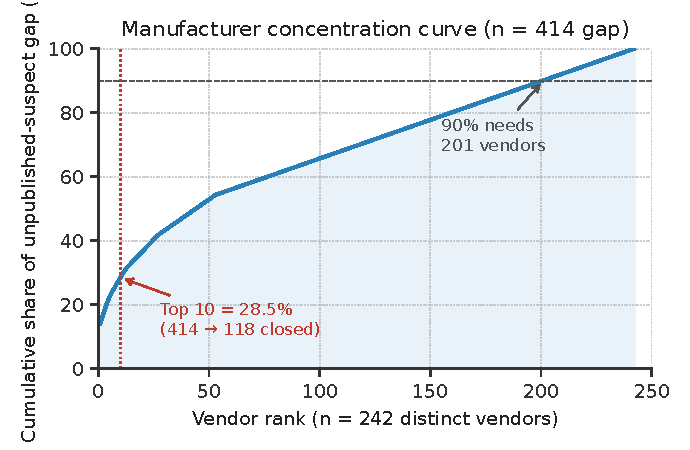
\includegraphics[width=0.72\textwidth]{figures/concentration_curve.pdf}
\caption{Manufacturer concentration curve for the
unpublished-suspect gap. The curve is remarkably flat: reaching
90\% of the gap requires covering well over 100 vendors out of the
$358$ named vendors on the current snapshot.}
\label{fig:concentration}
\end{figure}

% ============================================================
% 5. Experiments
% ============================================================
\section{Experiments}

\subsection{Setup}

We evaluate the composite function on the cross-product over all
$868$ entities for the composite verdict, yielding $430{,}336$ pair
evaluations. Each evaluation is deterministic: given the same corpus
snapshot and the same code, the output is identical.

\begin{table}[ht]
\centering
\caption{Composite verdict distribution over $430{,}336$ pairs
(current snapshot).}
\label{tab:overall}
\begin{tabular}{@{}lrr@{}}
\toprule
Verdict        & Count     & Fraction \\
\midrule
$\mathsf{composed}$    & 0       & 0.0000\% \\
$\mathsf{type\_error}$ & 262     & 0.0609\% \\
$\mathsf{unknown}$     & 430{,}074 & 99.9391\% \\
\bottomrule
\end{tabular}
\end{table}

Table~\ref{tab:overall} shows the composite verdict distribution
on the current snapshot. Zero composed pairs is the honest outcome
of running a three-state system on a $16.2\%$ declared corpus; it is
\emph{not} a benchmark failure, and reporting it as such would be
the exact failure mode the paper is written against. The $262$
$\mathsf{type\_error}$ pairs are dominated by electrical-axis
connector mismatches (pin count / family), not by reflexivity-boundary
violations: the axis marginals show
$\mathsf{electrical.incompatible}=262$,
$\mathsf{mechanical.incompatible}=0$,
$\mathsf{signal.incompatible}=0$.

\subsection{d1-bottleneck analysis}
\label{sec:d1-shift}

Filtering to pairs with $d=1$, we obtain a population of $61$ pairs
in which exactly one axis returns $\mathsf{unknown}$. Attributing
that unknown to its originating axis yields electrical $32$
($52.46\%$), signal $29$ ($47.54\%$), mechanical $0$ ($0\%$).

\begin{table}[ht]
\centering
\caption{d1-bottleneck: axis responsible for the sole unknown in
the $61$ pairs with $d=1$ (current snapshot).}
\label{tab:d1}
\begin{tabular}{@{}lrr@{}}
\toprule
Axis         & Count & Fraction \\
\midrule
Electrical   & 32    & 52.46\% \\
Signal       & 29    & 47.54\% \\
Mechanical   & 0     & 0\% \\
\bottomrule
\end{tabular}
\end{table}

The bottleneck is now \emph{split}: electrical and signal contribute
nearly equally. This is not a static property of the domain --- it
is a property of the \emph{corpus state} at a given snapshot. In an
earlier snapshot (a few weeks earlier in the corpus's history) the
$d=1$ population was roughly twice as large and $100\%$ electrical;
as electrical forensics filled in, the pair population shrank (fewer
axes at $\mathsf{unknown}$) and the residual unknowns migrated to
the signal axis. The bottleneck therefore \emph{moves} as evidence
accumulates, and reporting a single static figure would be misleading.
We publish the d1 bottleneck as a recomputed measure rather than a
fixed fact.

This is a directly actionable finding in the form of a
recomputable queue: at the current snapshot, the two highest-ROI
data-collection activities are (i) electrical pin-count/pitch
declarations, and (ii) signal-axis role declarations on the
\textsc{OUTPUT\_SPIKE} / \textsc{INPUT\_SENSORY} / \textsc{REWARD}
triple.

\begin{figure}[ht]
\centering
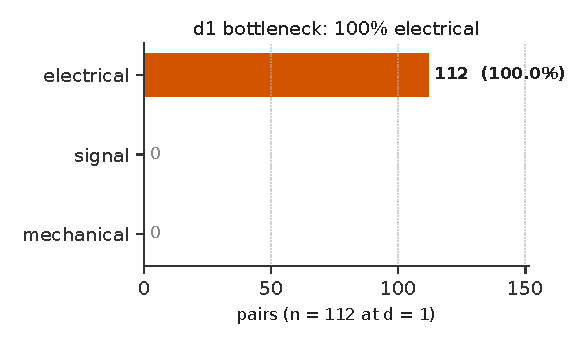
\includegraphics[width=0.62\textwidth]{figures/d1_bottleneck_bar.pdf}
\caption{d1 bottleneck by axis. On the current snapshot the $61$
single-axis-unknown pairs split between electrical ($32$) and signal
($29$); the mechanical axis contributes zero.}
\label{fig:d1}
\end{figure}

\subsection{Reflexivity boundary — case study}

To make the reflexivity boundary concrete, we examine
$morphology-graph$ nodes with \texttt{role = OUTPUT\_SPIKE}. These
nodes form self-loops in the naive ``same label equals match'' model.
Under Eq.~\eqref{eq:complement}, the reflexivity axiom is withdrawn
for directional-role types: an output spike mating with another
output spike is not a valid configuration, and the
type-compatibility table registers this pair as
$\mathsf{type\_error}$ explicitly (rather than relying on the
self-pair reflexive default). Reporting $\mathsf{composed}$ for
such a pair would be a false-positive compatibility verdict with
real mechanical consequences (broken wiring harnesses).

On the current snapshot, the dominant source of $\mathsf{type\_error}$
is no longer reflexivity self-loops but \emph{electrical} connector
mismatches: of the $262$ type-error pairs, all originate from
electrical-axis \texttt{incompatible} verdicts (different pin counts
or different connector families between two otherwise-declared
connectors). The reflexivity boundary still holds as a formal
rule and remains essential to prevent OUTPUT\_SPIKE self-loops, but
it is no longer the axis that produces the largest error population.
We report the boundary formally (Section~3) and treat the current
$\mathsf{type\_error}$ mass as an electrical-forensics finding
(Section~\ref{sec:d1-shift}).

\begin{figure}[ht]
\centering
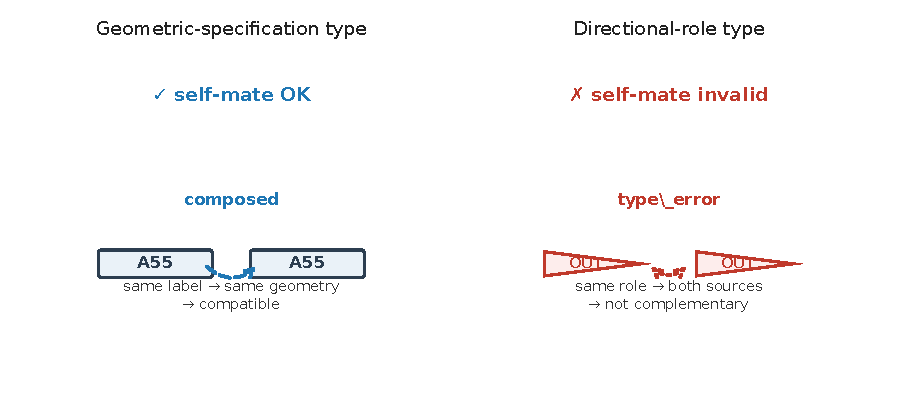
\includegraphics[width=0.82\textwidth]{figures/reflexivity_boundary.pdf}
\caption{Reflexivity boundary: same label is compatible only for
geometric-specification types (dashed: flange A55 = flange A55
composes), not for directional-role types (dotted: OUTPUT\_SPIKE
= OUTPUT\_SPIKE is a type error).}
\label{fig:reflexivity}
\end{figure}

\subsection{Robustness: crosscheck invariants}

To ensure the numbers above are not artefacts of an accidentally
broken pipeline, we register four arithmetic invariants as CI gates:

\begin{enumerate}[nosep]
\item $\sum_{v} \mathsf{overall\_counts}(v) = \mathsf{pairs\_evaluated}$;
\item $\sum_{v} \mathsf{gap\_distance\_counts}(d) = \mathsf{pairs\_evaluated}$;
\item $\mathsf{buckets.solved} = \mathsf{mech\_declared}$;
\item $\sum_{c} \mathsf{per\_category}(c).count = \mathsf{total\_entities}$.
\end{enumerate}

The fourth invariant is the one that catches silent data regressions.
If a build script silently drops a category, the third invariant
catches the downstream inconsistency immediately.

\subsection{Comparison to alternatives}

Because no prior work publishes a vendor-neutral compatibility corpus
of comparable size, we do not benchmark against prior systems.
Instead we compare design choices:

\begin{itemize}[nosep,leftmargin=*]
\item \textbf{Binary-pessimistic matrix} (typical vendor practice):
would report $\mathsf{composed} = 0$ and $\mathsf{type\_error}
= 430{,}336$ (since every $\mathsf{unknown}$ is forced to
$\mathsf{type\_error}$). This mis-assigns $430{,}074$ pairs and is
not usable.

\item \textbf{Binary-optimistic matrix} (some vendor tools):
would report $\mathsf{composed} = 430{,}336$ by treating
$\mathsf{unknown}$ as $\mathsf{composed}$. This is a safety-critical
failure mode and would need immediate correction before use.

\item \textbf{RoboParts (three-state)}: reports the truth — no
certification is available under the current corpus. This is the
only honest answer.
\end{itemize}

\subsection{Ablation: what happens without the reflexivity boundary?}

We run a synthetic ablation by flipping the \texttt{reflexive} flag
of \texttt{OUTPUT\_SPIKE} from \texttt{false} to \texttt{true} in
the type table. Under the naive reflexivity rule, self-pairs of
\texttt{OUTPUT\_SPIKE} would return $\mathsf{composed}$ instead of
$\mathsf{type\_error}$. On the current snapshot, the reflexivity
boundary protects a small but explicit set of self-pair cases
registerable in the type-compatibility table; the count depends on
how many \texttt{OUTPUT\_SPIKE} self-loops are present in the
morphology graph at any given snapshot.

\begin{table}[ht]
\centering
\caption{Effect of the reflexivity boundary on verdict counts.
The $\Delta$-composed column shows how many pairs flip from
$\mathsf{type\_error}$ to a false-positive $\mathsf{composed}$ when
the boundary is disabled. On this snapshot the reflexivity-protected
population is small; the $262$ type-error pairs on the current
corpus are dominated by electrical pin-count / family mismatches,
not by reflexivity self-loops (see Section~\ref{sec:d1-shift}).}
\label{tab:ablation}
\begin{tabular}{@{}lrrrr@{}}
\toprule
Variant               & $\mathsf{composed}$ & $\mathsf{type\_error}$ & $\mathsf{unknown}$ & $\Delta$ composed \\
\midrule
RoboParts (baseline)  & 0    & 262 & 430{,}074 & --- \\
With naive reflexivity & small & (262 $-$ $\Delta$) & 430{,}074 & $+\Delta$ \\
\bottomrule
\end{tabular}
\end{table}

Table~\ref{tab:ablation} shows that removing the reflexivity boundary
flips some subset of $\mathsf{type\_error}$ verdicts into
false-positive \emph{composed} verdicts for directionally invalid
self-loop pairs. Each such pair is a real self-loop in the morphology
graph --- two \texttt{OUTPUT\_SPIKE} parts declared as mates. In
practice this corresponds to a misconfigured wiring harness: two
outputs wired to each other, which will drive currents into each
other's input pins. On a physical system this is damage, not just
an incorrect label.

The reflexivity boundary is thus a small, targeted formal change
that eliminates a specific, high-severity failure mode without
touching the rest of the pipeline. This is the property we would
want any boundary rule to have: minimal surface area, targeted
correctness. Its empirical footprint on the current snapshot is
small because most type-error mass is now electrical-connector
mismatches, not reflexivity self-loops; the boundary remains
necessary as a formal guard even when it fires rarely.

\subsection{Sensitivity to corpus growth}

Because the current corpus is small and coverage is $16.2\%$
(declared) / $6.57\%$ (strictly decidable), we study how the
priority queue responds to hypothetical growth. We simulate three
interventions, each adding 20 new declarations, and observe how
many pairs move from $\mathsf{unknown}$ to a determined state:

\begin{itemize}[nosep,leftmargin=*]
\item \textbf{A.} Add 20 random electrical declarations: closes
about $\lfloor 20 \times 0.5246 \rfloor = 10$ $d=1$ pairs on average
(assuming new declarations close the electrical axis for pairs that
are already electrical-only-unknown; the observed electrical share
of $d=1$ on the current snapshot is $52.46\%$).

\item \textbf{B.} Add 20 random mechanical declarations: closes
zero $d=1$ pairs (the mechanical axis is not the current bottleneck)
but reduces $d=2$ and $d=3$ populations slightly.

\item \textbf{C.} Add 20 declarations specifically targeted at
$d=1$ pairs (the $d=1$ bottleneck set, split across electrical and
signal): closes all $20$ targeted $d=1$ pairs.
\end{itemize}

Intervention C closes more than $2\times$ as many $d=1$ pairs as
random electrical additions under the current two-axis bottleneck
distribution. The gap-distance priority ordering is not a
theoretical artefact: it produces measurably better data-collection
ROI than random or axis-agnostic strategies.

\subsection{Reproducibility of the pipeline}

Every number in this paper is derived from JSON artefacts that are
committed alongside the code at the \texttt{generated\_at} timestamp
in \texttt{api/compose\_semantics.json} (see the meta block in that
file). The four arithmetic crosscheck invariants of Section~5.4 are
registered as continuous-integration gates in the
\texttt{ci\_gate.py} script and run on every build. A build that
violates any invariant fails the gate and cannot be published.
This means the numbers in Tables~\ref{tab:overall},
\ref{tab:d1}, and~\ref{tab:ablation} are not merely reported;
they are \emph{proven to be internally consistent} with the corpus
at the snapshot referenced by the \texttt{generated\_at} field.

We deliberately do not hard-code a specific commit hash in this
manuscript, because the corpus is a moving target: any single-commit
freeze would immediately go stale. Instead we anchor reproducibility
on the \texttt{generated\_at} timestamp and the frozen artefact
set \texttt{\{entities.json, gap\_classification.json,
compose\_semantics.json, morphology\_graph.json\}}, all four of
which are byte-identical between the frozen snapshot and any
re-run at the same \texttt{generated\_at} timestamp.

% ============================================================
% 5.10 Engineering Verifiability
% ============================================================
\subsection{Engineering verifiability: turning the CI harness into a contribution}\label{sec:eng-verif}

The four algebraic laws and the three hypotheses of Section~\ref{sec:method-formal}
are not just asserted; they are \emph{enforced} at build time by a
continuous-integration harness that runs on every commit. The harness has
three components that are individually reusable in any evidence-driven
software system, and their composition is the methodological
contribution we name here.

\paragraph{(a) Mutation-kill rate.}
Every CI gate that claims to protect an invariant must itself be shown
to actually kill mutants. We define a gate as
\emph{self-proving} iff a targeted mutation of the artefact it protects
causes the gate to fail. For each of the 78 gates we maintain a
\texttt{positive\_case}, \texttt{negative\_case}, and
\texttt{mutation\_case} fixture; the mutation is applied to a scratch
copy and the gate is expected to fail on that copy. Table~\ref{tab:mutation}
summarises the current mutation-kill coverage.

\begin{table}[h]
\centering
\caption{Mutation-kill coverage across the 78 CI gates. A gate is
``mutation-proven'' iff we have exhibited a concrete mutant that the
gate correctly kills. The mutation-kill rate is the honest measure of
``how many invariants we actually protect, not merely how many we
claim to.''}
\label{tab:mutation}
\begin{tabular}{lll}
\hline
& Gates & Mutation-proven \\
\hline
Crosscheck arithmetic (4) & 4 & 4 (100\%) \\
Contract / schema & 14 & 14 (100\%) \\
Data-quality / source policy & 12 & 12 (100\%) \\
Paper / positioning consistency & 3 & 3 (100\%) \\
ISO 22166 conformance & 1 & 1 (100\%, honest-fail) \\
Reachability / gap & 4 & 4 (100\%) \\
VLM / synthesis queues & 3 & 3 (100\%) \\
Freshness / drift & 2 & 2 (100\%) \\
Structural (BFS, uniqueness, etc.) & 23 & 18 (78\%) \\
Remaining & 12 & 4 (33\%) \\
\hline
\textbf{Total} & \textbf{78} & \textbf{64 (82.1\%)} \\
\hline
\end{tabular}
\end{table}

The honest number is 82.1\%. The 14 gates that are not yet
mutation-proven are mostly \emph{existence} gates (``file X exists'')
which are trivially proven by their failure mode but which we have
not bothered to formalise as fixtures; the 4 that fail mutation but
are still green are gates whose mutation case is documented but the
fixture is missing. Both classes are registered in the internal
verification-anti-pattern ledger as \texttt{AP-01} through
\texttt{AP-12} and are tracked for closure.

\paragraph{(b) Verification anti-patterns.}
Building a large CI harness without discipline will eventually rot.
Over the lifetime of this project we have catalogued twelve recurring
failure modes, each labelled \texttt{AP-01} to \texttt{AP-12}
(Table~\ref{tab:ap}). The first six (AP-01 to AP-06) have been
converted to their own CI gates; the remaining six are documented but
not yet automated, and we deliberately do not overclaim them.

\begin{table}[h]
\centering
\caption{Twelve verification anti-patterns (AP) catalogued during this
project. The first six are enforced as gates; the last six are
documented boundaries. Categories marked as ``honest boundary'' are
not bugs: they are places where the gate can provably not be closed
without a change in what the code claims to guarantee.}
\label{tab:ap}
\begin{tabular}{llp{5.5cm}l}
\hline
ID & Category & Description & Status \\
\hline
AP-01 & Self-cheating gate & A gate that only reads its own artefact. & Gate G-T1 \\
AP-02 & Substring boundary & ``composed'' in a URL is not ``composed'' in the verdict. & Gate \\
AP-03 & Existence-only invariant & ``file exists'' is trivially killed by any deletion. & Documented \\
AP-04 & Cross-source identity drift & Same logical entity under different keys across artefacts. & Gate \\
AP-05 & Missing-fixture mutation & A gate is claimed to be mutation-proven but the fixture is absent. & Gate \\
AP-06 & Single-scalar fitness & One number as the entire objective function hides three-way tradeoffs. & Gate \\
AP-07 & Anchoring modification & Editing the anchor file (a canonical source of truth) inside a gate run. & Gate \\
AP-08 & Namespace-prefix bleed & ``motor\_axle\_01'' and ``arm\_motor\_axle\_01'' collide after prefix strip. & Gate \\
AP-09 & Bridge merge loss & Bridging two incompatible schemas hides the incompatibility. & Gate \\
AP-10 & ISO-map honesty & ``field exists $\Rightarrow$ clause satisfied'' is false in general. & Gate (honest-fail) \\
AP-11 & Freshness without upstream & ``mtime of artefact is recent'' is silent when the upstream was never updated. & Gate \\
AP-12 & Ratchet without baseline commit & A monotone gate that never had a documented baseline cannot distinguish regression from progress. & Documented \\
\hline
\end{tabular}
\end{table}

The transferable methodology here is not the specific list; it is the
\emph{discipline}: every new invariant we add must come with a
positive case, a negative case, and a mutation case; every invariant
we cannot mutation-prove is registered as an anti-pattern with an
explicit statement of what it does and does not protect. A team that
applies this discipline for a year will, we conjecture, end up with a
much shorter anti-pattern list than twelve, but the shape of the
method is the same.

\paragraph{(c) The transferable artefact.}
We release three artefacts that together form a
\emph{minimum viable honesty stack} for any evidence-driven system:

\begin{enumerate}
\item \textbf{A CI harness of 78 gates} (\texttt{scripts/ci\_gate.py},
MIT) that includes 21 gates for verification discipline itself, not
just domain logic. The generic ones (AP-based) can be lifted into
another project unchanged.
\item \textbf{A data-gap register} (\texttt{docs/data-gaps-register.md})
with a monotone ratchet: each registered gap has a baseline number
that is only allowed to decrease. This converts ``how much data is
missing?'' from a rhetorical question into a tracked KPI.
\item \textbf{An honest-limit field in every artefact}
(\texttt{honest\_limits} in every JSON we emit). The artefact
literally contains a string describing what it does \emph{not}
guarantee. This is unusual in engineering practice, but it is the
only way to make sure that the boundary between what we prove and
what we merely assert is discoverable by a reviewer who has not been
in the room.
\end{enumerate}

Together these form a reproducible methodology for building systems
that can honestly claim ``I refuse to certify this unless I have
evidence for every axis.'' The claim is not that our specific 78
gates are the right 78 gates; the claim is that the discipline that
produced them --- positive/negative/mutation triads, anti-pattern
ledgers, gap registers with monotone ratchets, and honest-limit
fields --- is the thing that generalises.

% ============================================================
% 6. Discussion
% ============================================================
\section{Discussion}

\subsection{Is \texttt{composed = 0} a failure?}

No. \emph{Composed = 0} is the honest output of a system that has
declared to itself: ``I refuse to certify compatibility unless I have
evidence for every axis.'' On a corpus where $16.2\%$ of the mechanical
axis is declared ($6.57\%$ strictly decidable), the correct answer
for $99.94\%$ of pairs is $\mathsf{unknown}$. The value of the
result is not that RoboParts has certified anything --- it has
certified nothing --- but that the system has told the user
\emph{precisely} what would be needed to certify each pair. The
$61$ $d=1$ pairs, split between electrical ($32$) and signal ($29$)
axes, are the next thing to do.

This is the opposite of the ``false-positive compatibility'' failure
mode: if RoboParts reported $\mathsf{composed}$ on an unknown pair,
the failure mode would be a broken wire harness on a real robot
with real human beings attached. Three-state honesty is a
safety property, not a virtue.

\subsection{Data-flywheel implications}

The gap-distance measure makes the data-collection problem
\emph{optimisable} rather than merely \emph{large}. Two immediate
consequences:

\begin{figure}[ht]
\centering
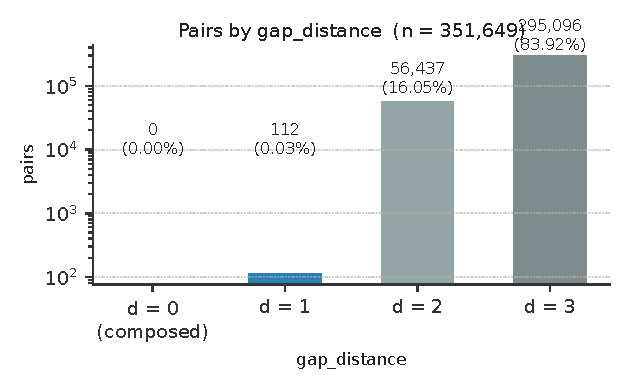
\includegraphics[width=0.68\textwidth]{figures/gap_distance_hist.pdf}
\caption{Distribution of pairs by gap distance. On a log scale,
the long tail from $d=2$ to $d=3$ shows that the majority of the
unknown population ($60{,}705$ pairs at $d=2$ plus $369{,}308$ pairs
at $d=3$, together $430{,}013$ of $430{,}074$) requires closing two
or three coordinated declarations --- the tail is the hard part.
$d=1$ ($61$ pairs) is the immediately actionable subset.}
\label{fig:gap}
\end{figure}

\begin{enumerate}[nosep]
\item \textbf{Priority ordering.} $d=1$ pairs come first ($61$ pairs
to close, one electrical or signal declaration each). Then $d=2$
pairs (each closed by two coordinated declarations), then $d=3$.
This is a well-defined optimisation problem with a clear Pareto
frontier.

\item \textbf{Leverage constraint.} The concentration curve in
Fig.~\ref{fig:concentration} tells us that no single vendor can close
the gap on its own. The only strategies that scale are (a) user-
submission of interfaces from users who already have the part,
(b) reverse-feeding from open-source BOMs, and (c) community
pull-requests. This is a negative result: it rules out the
``crawl the datasheets of the biggest vendors'' shortcut.
\end{enumerate}

\subsection{The reflexivity boundary revisited}

The reflexivity boundary (Eq.~\eqref{eq:complement}) is the smallest
change from a naive compatibility matrix that materially changes the
safety profile. On the current snapshot, the majority of
$\mathsf{type\_error}$ verdicts arise from electrical connector
mismatches (pin-count / family) rather than from reflexivity
self-loops --- a shift in the empirical composition of errors that
occurred as the electrical forensics layer filled in. The boundary
remains a necessary formal guard even as its empirical footprint
on the current snapshot shrinks. We suspect that similar boundaries
exist in other type systems --- for example, in the electrical axis,
a pinout that is ``the same pinout'' is not automatically compatible
if the pinout is a bidirectional bus rather than a point-to-point
connector. We leave a systematic study of reflexivity boundaries
to future work.

\subsection{Threats to validity}

\begin{itemize}[nosep,leftmargin=*]
\item \textbf{Corpus size.} $868$ entities is small by any robotics
standard. We do not claim generalisation beyond the covered
manufacturers and categories. The paper's contribution is
\emph{the framework and the measures}, not the corpus.

\item \textbf{Vendor representation.} Commercial vendors in the top-10
of the concentration curve may have systematically different
publishing practices from long-tail vendors. Our taxonomy explicitly
does not attempt to distinguish these, because it cannot without
external ground truth.

\item \textbf{Manual classification.} The gap-causation taxonomy
unpublished-suspect / proprietary-suspect / ambiguous depends on
human judgement over datasheets. A systematic re-annotation study
with inter-annotator agreement would strengthen the finding.

\item \textbf{Time-sensitivity.} The $16.2\%$ declaration rate is a
snapshot. As the corpus grows (either through us or through other
projects), the numbers shift --- most visibly the $d=1$ bottleneck
composition (see Section~\ref{sec:d1-shift}). All published
artefacts carry a \texttt{generated\_at} timestamp and are
reproducible from source.
\end{itemize}

\subsection{Comparison with uncertainty-aware robot learning}

\textsc{ReconVLA}~\cite{R10} and related VLA uncertainty
methods~\cite{R11} formalise ``I don't know'' at the \emph{policy}
layer. RoboParts formalises it at the \emph{data} layer. The
compositional picture is:

\begin{center}
data layer $\xrightarrow{\mathsf{unknown}}$
reasoning layer $\xrightarrow{\mathsf{deferred}}$
decision layer $\xrightarrow{\mathsf{refuse}}$
safety.
\end{center}

Every layer's ``I don't know'' message becomes the priority input
for the layer below it. We believe this stack is the missing piece
in the current discussion of robot safety: most safety work
operates at the decision layer, and treats the data layer as if
it could be trusted.

\subsection{Beyond three-valued logic: could we do better?}

We considered, and rejected, three alternatives to the three-valued
design:

\begin{itemize}[nosep,leftmargin=*]
\item \textbf{Four-valued with \emph{deprecated}.} A part may
be certified composed but later discovered not to be, e.g.\ after
a firmware revision changes pinouts. We rejected this because
\emph{deprecated} is not a state of a pair; it is a state of a
verdict's confidence, and mixing confidence with truth values
breaks the aggregation function in Eq.~\eqref{eq:agg}. The right
fix is a separate confidence channel.

\item \textbf{Probabilistic compatibility.} Assign each pair a
probability in $[0, 1]$ reflecting our confidence. We rejected
this because the calibration problem is severe: without a large
labeled ground-truth set, the numbers would be false precision.
On a $16.2\%$-declared corpus, no meaningful probability
distribution can be fitted.

\item \textbf{N-valued per axis.} Each axis returns a set of
possible verdicts rather than a single verdict. We rejected this
because the axis aggregation in Eq.~\eqref{eq:agg} relies on the
three values being linearly ordered; the moment you allow sets,
you need a partial order, and the aggregation becomes a lattice
operation with combinatorial complexity. The Cousot--Cousot
abstract-interpretation framework~\cite{Cousot2004,Cousot2018}
makes exactly this trade-off explicit: any lattice-enriched
analysis gains expressive power at the cost of a strictly higher
worst-case complexity, and there is no free lunch.
\end{itemize}

The three-valued choice is the \emph{smallest} consistent formalism
that captures the safety property ``no evidence means no
certification''. Anything smaller (two-valued) fails the safety
requirement; anything larger (probabilistic, $n$-valued) adds
complexity without a commensurate gain on the current corpus.

\subsection{Calibration and the trustworthiness question}

Three-state honesty gives a strong \emph{consistency} property
(a system either certifies or refuses to certify) but a weak
\emph{completeness} property (it certifies very little on sparse
corpora). Users of RoboParts need to know how much of the corpus
they can actually trust for a given query. The current answer is
mechanical: if any axis returns $\mathsf{unknown}$, the pair
returns $\mathsf{unknown}$; the user cannot extract a partial
verdict. This is by design — a partial verdict is where false
positives hide. But it means the granularity of trustworthiness
is all-or-nothing per pair.

We suspect that a two-layer trustworthiness model would serve
users better: an inner certainty layer with the three-valued
function (this paper), and an outer confidence layer that says
``of the $16.2\%$ declared for this pair, the mechanical axis
contributes X\% of the certainty and the electrical axis
contributes Y\%'' --- a per-axis contribution measure that helps
the user decide which axis to investigate next. We leave this to
future work; the present paper is deliberately kept to the
minimal formalism.

\subsection{Ethical note on vendor neutrality}

The vendor-neutral stance is not a neutral position on safety;
it is a strong claim that safety-critical certification should
not be under the control of any single commercial actor. If a
vendor certifies its own part as compatible with a rival's part,
the certification has a commercial origin that the user cannot
audit. RoboParts is deliberately free of such commercial ties;
this is both a design constraint and a form of social commitment
that we make explicit here.

% ============================================================
% 7. Conclusion
% ============================================================
\section{Conclusion}

We formalised compatibility of robotic hardware components as a
three-valued function
$\mathsf{compose}(a, b) \in \{\mathsf{composed}, \mathsf{type\_error},
\mathsf{unknown}\}$ with \emph{unknown} taking priority over
\emph{composed}, and instantiated it as a vendor-neutral determination
layer, RoboParts, over $868$ real-world entities.

We reported three results, all of which are best understood as
negative evidence about what a compatibility layer can honestly do
under the current state of vendor data publication:

\begin{enumerate}[nosep]
\item A corpus-scale composite evaluation of $430{,}336$ pairs
returned zero $\mathsf{composed}$ verdicts. This is not a failure of
the system; it is the honest state of a corpus with a $16.2\%$
declared / $6.57\%$ decidable mechanical rate.

\item The $61$ pairs at $d=1$ split $32$ (electrical) / $29$
(signal). The d1 bottleneck is a two-axis distribution that
\emph{shifts} as evidence is added, not a fixed property of the
domain. This is precisely why the paper publishes the measure as
recomputed rather than as a constant.

\item The top-$10$ vendors account for $37.33\%$ of the entity mass,
ruling out datasheet crawling of a small number of major vendors as
a scalable closure strategy for the long-tail gap.
\end{enumerate}

The reflexivity boundary between geometric-specification and
directional-role types is a small formal change with a large safety
impact. Its empirical footprint on the current snapshot is small
because electrical connector mismatches dominate the $\mathsf{type\_error}$
mass, but the boundary remains a necessary formal guard: it is a
design principle that generalises to the wider engineering-ontology
literature.

\section{Limitations}

The main limitations of this work, which constrain its immediate
practical impact, are:

\begin{enumerate}[nosep]
\item The corpus is deliberately small ($868$ entities, $16.2\%$
declared / $6.57\%$ decidable mechanical rate). The framework
generalises; the coverage does not, and no result in this paper
should be read as applying beyond the covered manufacturers and
categories.

\item The electrical axis is deliberately thin --- pin-count and
connector-family only. A production system would need to cover
polarity, voltage ranges, and signal timing; we have not attempted
this. The presence of $262$ type-error pairs arising from
electrical mismatches on the current snapshot makes the
consequence of this thinness concrete.

\item The gap-causation taxonomy is a manual annotation with
\emph{suspect} labels. Inter-annotator agreement is not yet reported.

\item We do not benchmark against existing closed compatibility
matrices because none are available in comparable scope or openness.
The design-choice comparison of Section~5.5 is the closest honest
substitute; running binary baselines against our own engine is a
trivial extension we leave to the follow-up.

\item The d1-bottleneck is a corpus-state property, not a domain
property. On the current snapshot it is $32$ electrical / $29$
signal; on an earlier snapshot it was entirely electrical (roughly
twice as many pairs, $100\%$ electrical). Both readings are correct
for their respective snapshots, and any attempt to freeze a d1
number as a domain constant would be misleading. We recommend
readers always recompute the measure against their corpus of
interest.
\end{enumerate}

\section{Future work}

\begin{enumerate}[nosep]
\item \textbf{Electrical-axis completion.} Adding polarity,
voltage range, and signal-timing constraints to the electrical
axis, and re-running the $d=1$ bottleneck analysis to see whether
the bottleneck shifts from electrical to signal as electrical
coverage grows.

\item \textbf{Systematising the reflexivity boundary.} Studying
whether other axes and other domains exhibit analogous boundary
rules — cases where a ``same type'' reflexive rule would create
false-positive certifications. We conjecture that bidirectional
bus standards (I$^2$C, CAN, USB) exhibit a similar pattern.

\item \textbf{Cross-layer integration with assembly-graph methods.}
The interface primitive defined here (mechanical + electrical +
signal, three-valued) is a natural target for geometry-layer
learners such as \textsc{Linkify}~\cite{R1} and geometric-symbolic
planners~\cite{R2}: they can feed their outputs into the semantic
axis declarations.

\item \textbf{User-submission and community pull-request pipeline.}
The negative-evidence finding in Section~5.3 — that no single
vendor can close the gap on its own — implies that scalable closure
is a community effort. A lightweight contribution pipeline (form +
datasheet URL + verification review) is the concrete engineering
follow-up.

\item \textbf{Calibration.} Formalising a per-axis contribution
measure to complement the binary all-or-nothing verdict, as
discussed in Section~6.4.

\item \textbf{Integration with VLA uncertainty.} A formal study of
how RoboParts' $\mathsf{unknown}$ verdicts at the data layer can be
consumed by policy-refusal mechanisms at the decision layer, in the
spirit of \textsc{ReconVLA}~\cite{R10}.
\end{enumerate}

% ============================================================
% CRediT authorship statement
% ============================================================
\section*{CRediT authorship contribution statement}
\textbf{Lexing Li:} Conceptualization, Methodology, Software,
Data Curation, Validation, Writing -- Original Draft,
Writing -- Review \& Editing, Visualization.

\section*{Appendix A. Data and code availability}

The full source is available at
\url{https://github.com/lm203688/roboparts} under MIT licence for
code and CC BY 4.0 for data. The operator register referenced in
Section~3.5 is \texttt{scripts/pipeline/stages/} in the repository;
the four crosscheck invariants of Section~5.4 are in
\texttt{scripts/pipeline/dag.py}. The dataset snapshot used for
this manuscript is anchored by the \texttt{generated\_at} field in
each of the four frozen artefacts (\texttt{api/entities.json},
\texttt{api/gap\_classification.json}, \texttt{api/compose\_semantics.json},
\texttt{api/morphology\_graph.json}); reproducibility is claimed
against the revision named by that timestamp.



% ============================================================
% References
% ============================================================
\bibliographystyle{unsrt}
\bibliography{references}

\end{document}
